\chapter{Dise\~no del sistema de distribución de carga}
\label{cap:disenoSistema}

Como se había mencionado en la subsección \ref{intro:problema}, el problema de la sobrecarga en un SPS está arraigado por la inflexibilidad que posee el grafo diseñado. Esto quiere decir, que en el momento que el sistema está funcionado, cambia la cantidad de recursos necesarios en el sistema, por lo que puede volver ineficiente o sobrecargado el sistema.

De ser así, el sistema necesita un sistema que pueda proveer dinamismo en su estructura, así como también análisis de la carga tanto en el momento como a futuro, de tal manera que se complementen. De tal manera de diseñar un sistema de bajo costo que pueda optimizar su rendimiento, sin generar interrupciones en la ejecución del sistema.

\section{Análisis del sistema de distribución de carga}
Dentro del análisis realizado en la arquitectura del sistema implementando, se consideró una perspectiva en base a los recursos lógicos según el enfoque dinámico, definido en las subsección \ref{subsec:recLogicosBC} y \ref{subsec:enfoqueDinamicoBC} respectivamente, para el balance de carga de SPS. Esto debido que el trabajo presentando no analizó el comportamiento que tenga cada uno de los nodos del sistema, sino que se analizó el rendimiento que poseía cada uno de los operadores del grafo diseñado en base a un SPS.

Respecto al estudio de las distintas técnicas implementadas, era necesario utilizar una que no tuvieran desventajas en cuanto a la pérdida de datos, inadaptabilidad con el tiempo y costo de implementación. Por lo tanto, se consideró que la mejor opción era utilizar la técnica de fisión, utilizando el mismo modelo de replicación que Fernández \citep{FernandezMKP13}, donde según una sobrecarga en el operador era necesario generar una replica de ese operador. Dentro de las hipótesis planteadas, se pensaba que el costo de un operador iba a ser menor a la formación de las colas de datos en el sistema, lo cual podría variar según la arquitectura del SPS implementando.

Para el diseño del sistema, era necesario contar con un umbral que determinara cuando el operador está o no sobrecargado, por lo que para esto se utilizaron conceptos de teoría de colas \citep{bose2013introduction}. Como los SPS están orientados en grafos, se posee tanto la tasa de llegada ($\lambda$) como la tasa de procesamiento ($\mu$) para cada uno de los operadores, como se ve representando en la Figura \ref{fig:analisisTeoriaColas}, donde la tasa de procesamiento de un operador es la misma tasa de llegada del siguiente operador en el grafo. Utilizando este tipo de conceptos, para cada operador se calculó la tasa de procesamiento ($\rho$), la cual esta definida por la tasa de llegada, la tasa de procesamiento y la cantidad de servicios disponibles en el sistema ($\rho = \frac{\lambda}{\mu \rho}$), cuyo valor nos indica el rendimiento del operador en cierta período de tiempo.

Dado este tipo de enfoque y la elasticidad que se deseaba por parte del sistema, es que se trataron tres tipos de estados que pudieran surgir en el sistema: ocioso, estable e inestable. El primer estado hace referencia a cuando el sistema posee mayor cantidad de recursos de lo necesario. El segundo es cuando el sistema se encuentran en un rendimiento óptimo. Y por último, el tercero hace referencia a cuando el sistema posee una sobrecarga, por lo que necesita una mayor cantidad de recursos. Definido el estado del sistema, se tomó esto como la base para las funciones que iban a desempeñar los componentes de análisis y predicción de carga.

\begin{figure}[!hb]
	\centering
		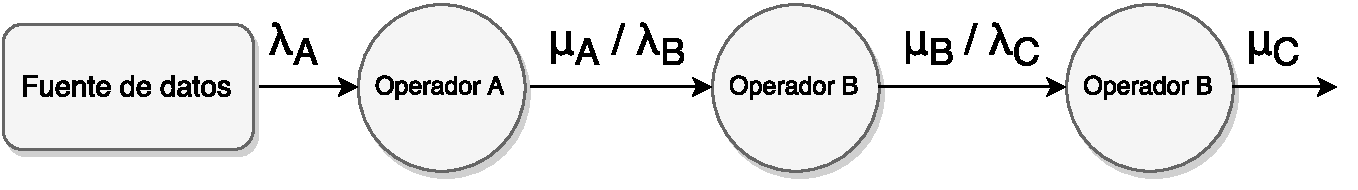
\includegraphics[scale=0.6]{images/AnalisisTeoriaColas.pdf}
	\caption{Enfoque de un SPS con conceptos de teoría de colas.}
	\label{fig:analisisTeoriaColas}
\end{figure}

Por último, se consideró importante tratar con dos tipos de algoritmos, uno enfocado en el presente y otro en el futuro. Esto fue pensando, debido que el análisis en el presente no iba a encontrar algún patrón o \textit{peak} que indicara que iba a poseer el mismo comportamiento a futuro, a diferencia de algún algoritmo predictivo. Esto se puede ver ejemplificado en curvas exponenciales, dado que si la tasa de llegada de los datos va aumentando exponencialmente, es necesario ir aumentando paralelamente los recursos del sistema para no generar una sobrecarga. Pero, en caso que falle la predicción, existe el algoritmo reactivo que podrá mejorar el rendimiento en el momento.

Al considerarse un sistema que pudiera lidiar con dos tipos de algoritmos, era necesario considerar un algoritmo que pudiera administrar la cantidad de cargas, con tal analizar el algoritmo a utilizar según el tiempo, como también la cantidad de réplicas que deben aplicarse.

Dado lo anterior, se diseño un sistema de distribución de carga con cuatro componentes: monitor de carga, analizador de carga, predictor de carga y administrador de réplicas, que se pueden apreciar en la Figura \ref{fig:componentesSistemas}.

\begin{figure}[ht!]
  \centering
    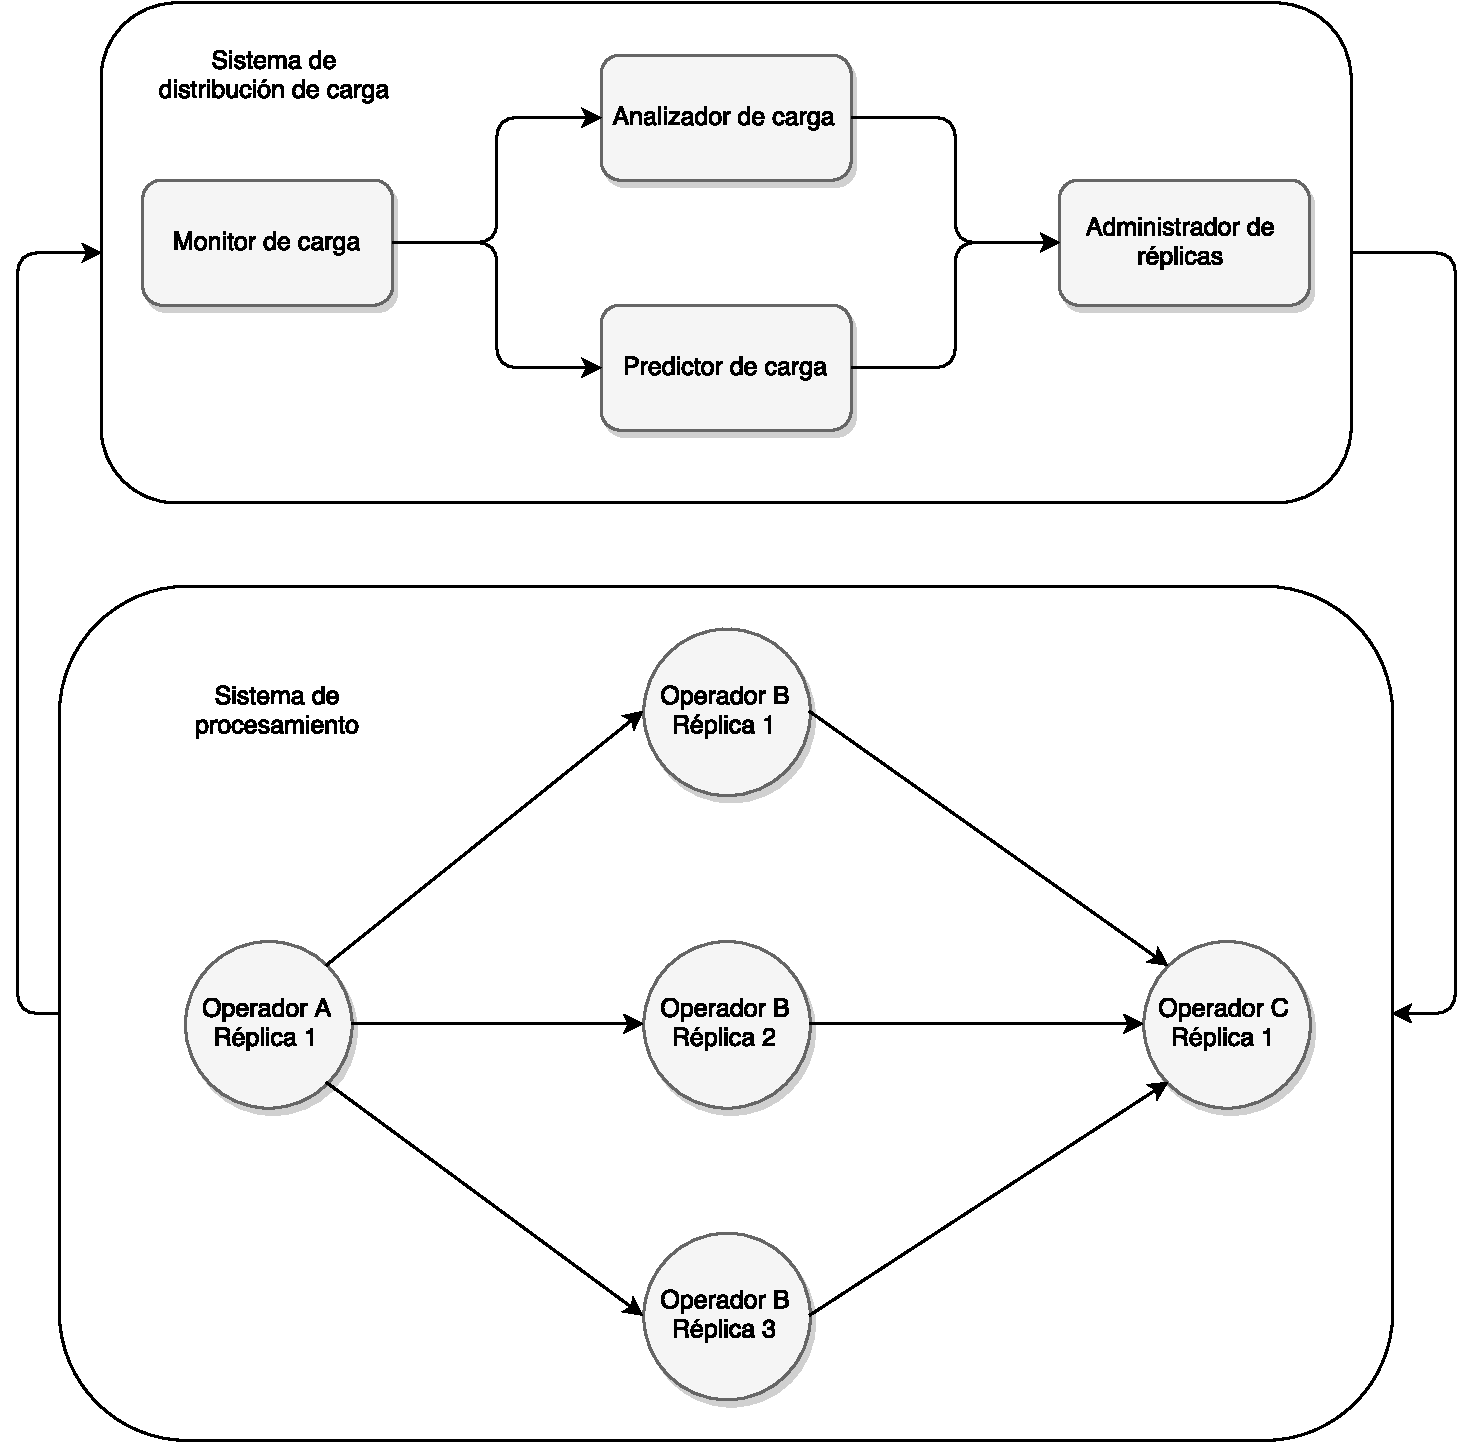
\includegraphics[scale=0.5]{images/Diagrama.pdf}
  \caption{Estructura del sistema de distribución de carga.}
  \label{fig:componentesSistemas}
\end{figure}

\paragraph{Monitor de carga} Está encargado de estar enviado las estadísticas al sistema, ya sea para recolectar las estadísticas para el algoritmo reactivo como predictivo.

\paragraph{Analizador de carga} Verifica cual es la carga cada cierto período de tiempo, y respecto a eso indica si debe o no replicarse. Para esto, se considera el rendimiento de cada operador, de esta manera se compara el valor del rendimiento con el umbral propuesto, y según en que rango esté va a ser el estado que se encuentren, el cual indica si debe disminuir, aumentar o mantenerse la cantidad de réplicas.

\paragraph{Predictor de carga} Realiza una predicción en base a la historia realizada en cierta ventana de tiempo, utilizando como base las cadenas de Markov. De esta manera, se realiza un cálculo de la distribución estacionaria \citep{Papoulis1984}, para determinar el estado del sistema a futuro y tomar una decisión respecto a esto.

\paragraph{Administrador de réplicas} Es quién administra la cantidad de réplicas de un operador en específico, y además cual de los modelos será utilizado.

\section{Recolección de los datos}
Como se había mencionado anteriormente, el monitor de carga está encargado de recolectar la tasa de rendimiento de cada uno de los operadores, tanto del historial como los datos en el momento. Para esto, se consideró una ventana de tiempo de 1 segundo para la recolección del historial, y 5 segundos para el análisis del operador en el momento.

Para la recolección del historial se consideraron muestras de 100 datos, esto fue propuesto de esta manera, debido que cada 100 segundos se realiza el algoritmo predictivo, tomando en consideración que cada un segundo recolecta una muestra. La cantidad de muestras fue determinado de esta manera, porque se consideró un número apropiado según lo indicado en la literatura \citep{ching2006markov}.

En cambio, para el algoritmo reactivo, se consideran datos del momento, los cuales son obtenidos cada cinco segundos. Con esta tasa de rendimiento, el algoritmo debe analizar si es necesario o no realizar alguna modificación al sistema, es importante destacar que no siempre es necesaria, debido que en cierto período sólo se utiliza el algoritmo predictor y no el reactivo. Dentro de las consideraciones que se hicieron, es realizar un promedio de la tasa de servicio ($\mu$) en cierta ventana de tiempo, de tal manera de poseer un dinamismo en el valor del procesamiento de los datos en el operador. Un ejemplo de esto, es que puede ser que en cierto período de tiempo se procesen datos más pesados que en otro período de tiempo, llegando la misma tasa de llegada, por lo que las tasas de procesamiento son distintas. Al realizar promedios en períodos de tiempos, las tasa de procesamiento irá adaptándose con el dinamismo de los datos.

\section{Algoritmo reactivo}
Para el diseño del algoritmo reactivo, como se expresó al inicio del capítulo, se tomó en cuenta conceptos de teoría de colas, por lo que la tasa de rendimiento es el factor que se utilizó para el análisis del estado del sistema.

Dentro de las definiciones de los algoritmos reactivos \citep{CasavantK88}, es necesario considerar umbrales para determinar el estado del sistema, el cual en este caso la tasa de rendimiento ($\rho$), por lo que según su valor el operador toma cierto estado. En el Algoritmo \ref{alg:reactive} se puede ver el análisis del estado de un operador según su tasa de rendimiento; en el caso que sea mayor a 1, su estado es inestable, menor a 0.5, significa que está en estado ocioso, y sino, significa que está estable. Estos datos posteriormente serán considerados por al administrador de réplicas, el cual analiza el comportamiento que debe tener el sistema según lo indicado por el algoritmo.

\begin{algorithm}[!ht]
	\caption{Algoritmo reactivo del sistema de distribución de carga.}
	\label{alg:reactive}
	\begin{algorithmic}[1]
	\REQUIRE Tasa de procesamiento $\rho$ del operador $\phi$.
	\ENSURE Estado del operador, donde -1 significa estado ocioso, 0 estable y 1 inestable.
	\IF {$\rho_\phi > 1$}
		\RETURN{1}
	\ELSIF {$\rho_\phi < 0.5$}
		\RETURN{-1}	
	\ELSE
		\RETURN{0}
	\ENDIF
	\end{algorithmic}
\end{algorithm}

En la Figura \ref{fig:umbrales} se muestra un ejemplo de la tasa de procesamiento, que en los primeros segundos el sistema está superior al límite superior, el cual indica que el sistema es inestable. Por lo que el sistema detecta dicha sobrecarga, e indica este problema, para que posteriormente en los 100 segundos pueda estabilizarse el sistema y quedarse entre el límite superior e inferior, el cual esta definido como sistema estable.

\begin{figure}[hb!]
  \centering
    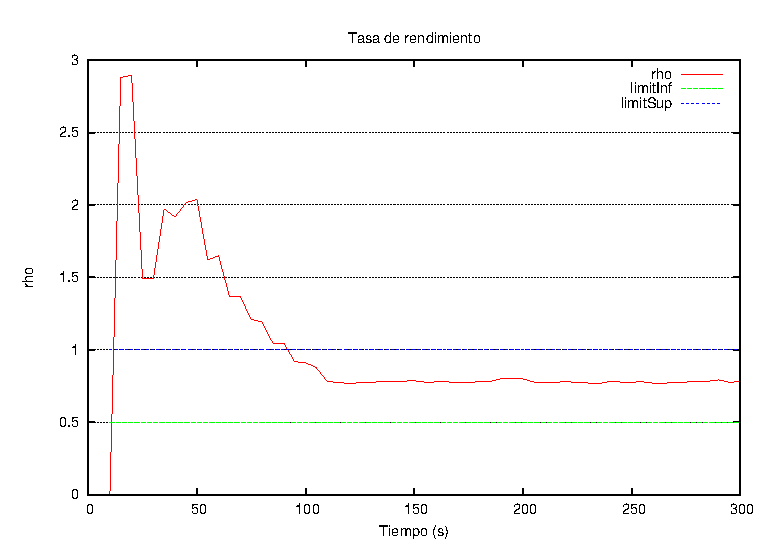
\includegraphics[scale=0.8]{images/Umbrales.eps}
  \caption{Estados de la tasa de procesamiento.}
  \label{fig:umbrales}
\end{figure}


\section{Algoritmo predictivo}
Para la confección del algoritmo predictivo se realizó un análisis según las cadenas de Markov \citep{ching2006markov}, por lo que es importante considerar las siguientes condiciones necesarias:

\begin{itemize}
	\item Definir tiempo discretos, los cuales fueran cambiando con el tiempo según un proceso estocástico. Para esto se consideró el cambio del estado del sistema de período a otro, es decir, las transiciones existentes entre cada uno de los estados, ya sea ocioso, estable o inestable, en período de un segundo.
	\item Determinar los estados finitos que se van a utilizar para la conformación de la cadena, que en este caso sería los estados que puede encontrar el sistema, siendo tres los posibles estados: ocioso, estable o inestable.
	\item Una cantidad de muestras considerables para realizar un muestreo que sea representativo según el período analizado, que en este caso fueron 100 muestras, las cuales corresponden a la tasa de rendimiento del operador analizado. Estas muestras serán independientes unas con otras, por lo que cada cierto período de tiempo se volverá a crear otra cadena de Markov independiente de los datos del pasado.
\end{itemize}

Dato esto, se presentó un cadena de Markov en base a estas bases, como se refleja en la Figura \ref{fig:cadenaMarkovPredictiva}, donde existen tres estados, los cuales pueden ser ocioso, estable o inestable, y poseen ciertas transiciones de un estado a otro, cuyas probabilidades van a estar determinadas por la historia existente en el sistema.

\begin{figure}[hb!]
  \centering
    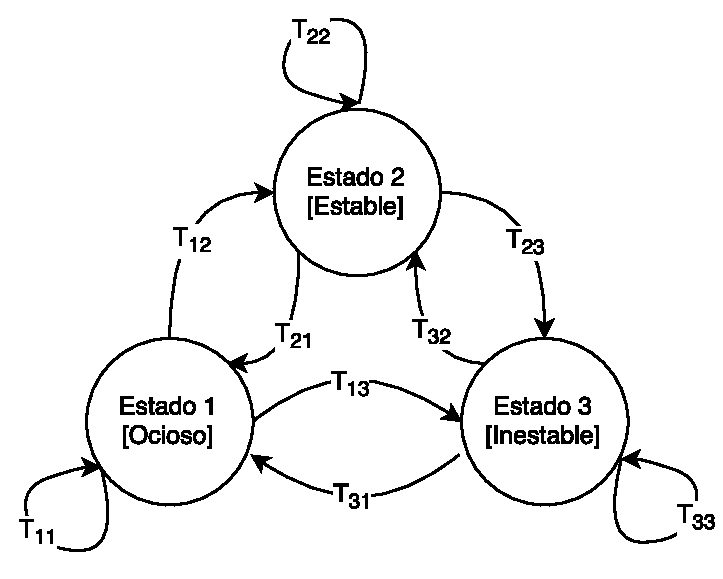
\includegraphics[scale=0.75]{images/CadenaMarkovPredictiva.pdf}
  \caption{Cadena de Markov dado el modelo propuesto del sistema.}
  \label{fig:cadenaMarkovPredictiva}
\end{figure}

Por lo tanto, para cada operador existe una cadena de Markov según la historia existente en una ventana de tiempo. Para la generación de esta cadena de Markov, se puede ver en el Apéndice \ref{apendice:matrizTransicion} el algoritmo que crea la matriz de transición según el historial del operador, la cual corresponde a la tasa de rendimiento recolectada cada un segundo en la última ventana de tiempo del operador analizado. En la Ecuación \ref{eq:matrizTransicionPredictive} se puede ver la matriz de transición que se obtiene de la cadena de Markov de la Figura \ref{fig:cadenaMarkovPredictiva}, la cual posee una probabilidad de transición desde cada uno de los estado a otro existente.

\begin{equation} \label{eq:matrizTransicionPredictive}
	P =
	\begin{bmatrix}
		T_{1,1} & T_{1,2} & T_{1,3} \\
		T_{2,1} & T_{2,2} & T_{2,3} \\
		T_{3,1} & T_{3,2} & T_{3,3}
	\end{bmatrix}	
\end{equation}

Teniendo la matriz de transición de la cadena de Markov de un operador, se puede calcular la distribución estacionaria, la cual indica la probabilidad que a largo plazo se encuentre el sistema en cierto estado, ya sea ocioso, estable o inestable. Para el cálculo de esta, se utiliza la ecuación de Chapman-Kolmogórov \citep{Papoulis1984} expuesta en la subsección \ref{subsec:cadenaMarkov}.

El Algoritmo \ref{alg:distEstacionaria} describe el cálculo de la distribución estacionaria, cuya entrada es la distribución estacionaria de un operador del SPS. Dentro de las primeras condiciones, era analizar si efectivamente existían transiciones en todos los estados, debido que podía darse que no existiera alguna transición a algún estado en un período de tiempo. Por ejemplo, podría ser que en cierto período nunca se ha encontrado ocioso el sistema, pero si estable e inestable. Como el cálculo de la distribución estacionaria requiere un estado de inicio, se verificó si efectivamente existía o no el estado, y en caso no existir, el estado de inicio será alguno existente.

Al realizar las iteraciones correspondientes a cálculo, se proporcionó como entrada la cantidad que se estimaba necesario. Es importante destacar que entre mayor cantidad de iteraciones, mayor precisión existe en el cálculo, pero mayor es el tiempo de espera.

\begin{algorithm}[!ht]
	\caption{Cálculo de la distribución estacionaria de la cadena de Markov de un operador $\phi$.}
	\label{alg:distEstacionaria}
	\begin{algorithmic}[1]
	\REQUIRE $\Gamma$ Matriz de transición del operador $\phi$ y $\upsilon$ cantidad de iteraciones deseadas.
	\ENSURE $\Delta$ Distribución estacionaria de la cadena de Markov del operador $\phi$.
	\STATE $i \leftarrow 0$ \COMMENT {Estado inicial de iteración}
	\FOR {$j=1$ a $3$}
		\IF {$\Gamma_{j,x} = 0 ; x={1,2,3}$}
			\STATE {$i \leftarrow j$}
		\ENDIF
	\ENDFOR
	
	\STATE $\tau \leftarrow Arreglo[3]$ \COMMENT {Contador para la normalizaci\'on de los datos}
	\FOR {$k=0$ a $\upsilon$}
		\STATE $u = randomUniform(0,1)$
		\STATE $\sigma = 0$
		\FOR {$j=0$ a $3$}
			\STATE $\sigma = \sigma + \Gamma_{i,j}$
			\IF {$u \leqslant  \sigma$}
				\STATE $\tau_{j}++$
				\STATE $i \leftarrow j$
				\STATE \textbf{break}
			\ENDIF
		\ENDFOR
	\ENDFOR

	\STATE $\Delta \leftarrow Arreglo[3]$ \COMMENT {Distribución estacionaria de la cadena de Markov del operador $\phi$}
	\FOR{$k=0$ a $3$}
		\STATE $\Delta_{k} \leftarrow \nicefrac{\tau_{k}}{\upsilon}$
	\ENDFOR	
	
	\RETURN $\Delta$
	
	\end{algorithmic}
\end{algorithm}

Obtenida la distribución estacionaria, se procese a analizarla el comportamiento de esta. Para esto, se consideró que era importante que la probabilidad entre estados tuviera una desviación estándar superior a 0.25, de tal manera que se trabajen con probabilidad que no posean incertidumbre en su comportamiento a futuro. En el Algoritmo \ref{alg:predictive} se puede ver el análisis que se realiza a la distribución estacionaria, ya sea por el comportamiento estadístico o de estado del sistema, donde retornará el estado a futuro del operador, dada la probabilidad más alta de la distribución estacionaria, si es que supera la desviación estándar propuesta. Se tomó en consideración que el primer estado es el ocioso, el segundo estado es el estable y el tercer estado es el inestable.

\begin{algorithm}[!ht]
	\caption{Algoritmo predictivo del sistema de distribución de carga.}
	\label{alg:predictive}
	\begin{algorithmic}[1]
	\REQUIRE$\Delta$ Distribución estacionaria de la cadena de Markov del operador $\phi$.
	\ENSURE Estado a futuro del operador, donde -1 significa estado ocioso, 0 estable y 1 inestable.
	\IF {$\sigma(\Delta_1,\Delta_2,\Delta_3) > 0.25$ \COMMENT {Desviaci\'on est\'andar de las probabilidades de la distribuci\'on estacionaria}} 
		\STATE $i \leftarrow getStateMax(\Delta)$ \COMMENT {Obtención del estado con mayor probabilidad}
		\IF {$i=1$}
			\RETURN -1
		\ELSIF {$i=2$}
			\RETURN 0			
		\ELSE
			\RETURN 1
		\ENDIF
	\ENDIF
	
	\RETURN 0
	
	\end{algorithmic}
\end{algorithm}

\section{Administración del sistema}

El último componente del sistema es el administrador de réplicas, cuya función es administrar la cantidad de réplicas en cada uno de los operadores según los recursos disponibles por parte del sistema y también según el comportamiento que éste posea.

Para esto, se diseño un administrador que se ejecutara según el período que se encuentra el algoritmo reactivo o predictivo, cada período es de 19 ejecuciones del algoritmo reactivo y 1 del algoritmo reactivo. Esto fue pensando dado que cada 100 segundos se poseían las muestras suficientes para el análisis del algoritmo predictivo, por lo tanto, cada ejecución del algoritmo reactivo iba a ser cada 5 segundos, de esa manera al segundo 100 iba a realizarse en vez del algoritmo reactivo, el predictivo ya que posee la cantidad suficiente de muestras.

\begin{algorithm}[!hb]
	\caption{Administración de réplicas de un operador $\phi$ dado su comportamiento en el sistema de distribución de carga.}
	\label{alg:administracion}
	\begin{algorithmic}[1]
	\REQUIRE Operador $\phi$ a analizar y $\iota$ período en que se encuentra el sistema de distribución de carga.
	\ENSURE Cantidad de réplicas a modificar del operador.	
	
	\IF {$\iota \mod{20} \neq 0 $}
		\STATE $\delta_{\iota} \leftarrow AlgoritmoReactivo(\phi)$
		\IF {$\delta_{\iota}$ \AND $\delta_{\iota-1}$ son estado inestable}
			\IF {No excede la cantidad máxima de réplicas en el sistema}
				\RETURN Crear una réplica del operador $\phi$
			\ENDIF
		\ELSIF {$\delta_{\iota}$ \AND $\delta_{\iota-1}$ son estado ocioso}
			\RETURN Remover una réplica del operador $\phi$
		\ENDIF 
	\ELSE
		\STATE $\delta_{\iota} \leftarrow AlgoritmoPredictivo(\phi)$
		\IF {$\delta_{\iota}$ es estado inestable}
			\IF {No excede la cantidad máxima de réplicas en el sistema}
				\RETURN Crear cinco réplicas del operador $\phi$
			\ENDIF
		\ELSIF {$\delta_{\iota}$ es estado ocioso}
			\RETURN Remover cinco réplicas del operador $\phi$
		\ENDIF
	\ENDIF
	
	\RETURN No hacer nada al operador $\phi$
	
	\end{algorithmic}
\end{algorithm}

En el Algoritmo \ref{alg:administracion} está el procedimiento de administración, donde primero se analiza si debe realizarse según el período el algoritmo reactivo o el predictivo. En caso de realizarse el reactivo, se analiza si existen dos alertas consecutivas del mismo estado del sistema, ya sea ocioso o inestable, y de ser así, realizar una modificación a la cantidad de réplicas del operador. Por otra parte, de ejecutarse el módulo predictivo, se analiza cual fue la predicción, por lo que si es ocioso disminuirá la cantidad de réplicas y si es inestable las aumentará. Como el proceso de predicción se realiza con menor frecuencia, se considero que debía crear o remover mayor cantidad de réplicas que en el módulo reactivo, con tal de aprovechar el costo de cómputo que conlleva éste.

Dentro de las consideraciones que se tuvieron para el diseño del administrador, fue la cantidad máxima de réplicas que podían realizarse. Dado que una de las limitantes de este trabajo fue que sólo se utilizó una máquina, la cantidad de recursos son limitados, por lo que aumentar la cantidad de réplicas indefinidamente iba a generar una sobrecarga en los recursos disponibles por parte de la máquina, habiendo fallas en el funcionamiento del SPS.